\subsection{To Merge Material}
\begin{frame}
Old Presentation.
    
\end{frame}
\begin{frame}
\thetitle{Optimization Strategy: Coordinate Ascent}
\[ \argmax_{\theta, \lambda} \sum_{n=1}^N \ELBO(\theta, \lambda; x^{(n)}) \]
Randomly initialize $\theta^*, \lambda^*$, then repeat:
\begin{enumerate}
    \item $\displaystyle \theta^* = \argmax_\theta \sum_{n=1}^N \ELBO(\theta, \lambda^*; x^{(n)})$
    \item $\displaystyle \lambda^* = \argmax_\lambda \sum_{n=1}^N \ELBO(\theta^*, \lambda;x^{(n)})$
\end{enumerate}
\begin{center}
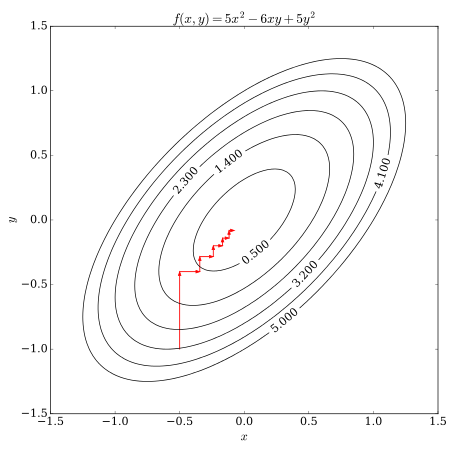
\includegraphics[scale=0.3]{pics/coordasc.png}
\end{center}

%Can be generalized in many ways:
%\begin{itemize}
%    \item Approximate $\argmax$
%    \[ a^{(i+1)} = a^{(i)} + \eta \nabla_a f(a^{(i)}, b^{(i)})\]
%    \item Block coordinate ascent
%\end{itemize}
\end{frame}

\begin{frame}
\thetitle{Preview}
\vspace{-4mm}
\begin{table}[]
    \centering
    \small
    \begin{tabular}{l c c c }
    \toprule
        Optimization Strategy  & $q$ &  $\max_\lambda$ & $\max_\theta$ \\
    \midrule
         Log Marginal Likelihood & - & - & Grad \\
         Expectation Maximization & Posterior & Bayes & Closed \\
         Variational EM &  Factored & Coord. & Closed \\
         Stochastic Variational EM  & Factored  & Grad & Grad\\
         Variational Autoencoder & Amortized & Grad & Grad \\
         \bottomrule
    \end{tabular}
\end{table}
\vspace{-2mm}
\textbf{$q$ Family examples} \\
Posterior: $q(z\param \lambda)$ matches $p(z \given x)$\\
Factored: e.g. $q(z^{(n)}) = \prod_{t} q(z^{(n)}_t\param \lambda^{(n)})$ \\
Amortized: e.g. $q(z^{(n)}) = \text{NN}(x^{(n)}\param \lambda)$  \\
\textbf{$\lambda$ Optimization Methods} \\
Bayes Rule: $q(z;\lambda) = p(z \given x )$ \\
Coordinate: $\lambda^{(n)*}_t = \argmax_{\lambda^{(n)}_t} \ELBO(\theta, \lambda^{(n)} \param x^{(n)}) $ \\
Gradient:\ $\lambda = \lambda + \eta \nabla_\lambda \ELBO(\theta, \lambda)$ \\
\end{frame}

\begin{frame}
\begin{tikzpicture}
% nodes
\node (dots) {$\ldots$};%
 \node[latent] (z) {$y^{(n)}$};%
 \node[const, right=of z] (x) {$x^{(n)}$};%
 %\node[obs, right=1cm of dots] (xT) {$x_T^{(n)}$};%
 \node[const, above=of z] (pi) {$\mathbf{w}$};
% plate
 \plate {plate1} {(z)(x)} {$N$}; %
 \edge{pi}{z};
 \edge{x}{z};
 
\end{tikzpicture}
    
\end{frame}

\begin{frame}{Frame Title}
    \begin{center}
\begin{tikzpicture}
% nodes
\node (dots) {$\ldots$};%
 \node[latent] (z) {$z^{(n)}$};%
 \node[const, right=of z] (x) {$x^{(n)}$};%

 %\node[obs, right=1cm of dots] (xT) {$x_T^{(n)}$};%
 \node[const, above=of z] (pi) {$\lambda$};
% plate
 \plate {plate1} {(z)(x)} {$N$}; %
 \edge{pi}{z};
 \edge{x}{z};
 
\end{tikzpicture}
\begin{tikzpicture}
% nodes
\node (dots) {$\ldots$};%
 \node[latent] (z) {$z^{(n)}$};%
 %\node[obs, right=1cm of dots] (xT) {$x_T^{(n)}$};%
 \node[const, above=of z] (pi) {$\lambda^{(n)}$};
% plate
 \plate {plate1} {(z)(pi)} {$N$}; %
 \edge{pi}{z};
\end{tikzpicture}
\begin{tikzpicture}
% nodes
\node (dots) {$\ldots$};%
 \node[latent] (z) {$z_1^{(n)}$};%
 \node[latent, right= of z] (zT) {$z_T^{(n)}$};%

 %\node[obs, right=1cm of dots] (xT) {$x_T^{(n)}$};%
 \node[const, above=of z] (pi) {$\lambda_1^{(n)}$};
\node[const, above=of zT] (piT) {$\lambda_T^{(n)}$};
%
% plate
 \plate {plate1} {(z)(pi)(piT)(zT)} {$N$}; %
 \edge{pi}{z};
 \edge{piT}{zT};
\end{tikzpicture}
\end{center}

\end{frame}

%\begin{frame}
%\thetitle{Optimization Strategy: Coordinate Ascent}
%\center
%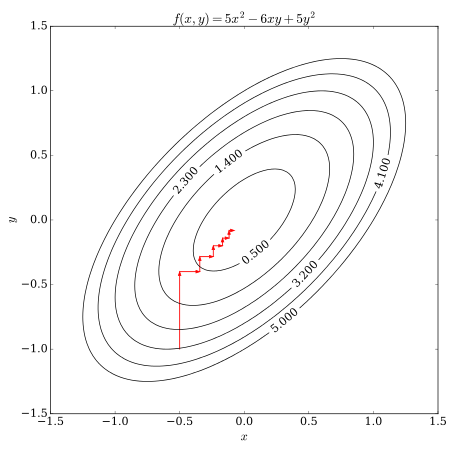
\includegraphics[scale=0.4]{pics/coordasc.png}
%\\
%(from {\footnotesize \url{https://en.wikipedia.org/wiki/Coordinate_descent}})
%\end{frame}

%\begin{frame}
%\thetitle{Coordinate Ascent on the ELBO}
%Aggregate ELBO
%\[ L(\theta, \lambda^{(1)}, \dots, \lambda^{(N)}) =  \sum_{n=1}^{N} \ELBO(\theta, \lambda^{(n)} \param x^{(n)}) \]
%Repeat:
%\begin{enumerate}
%\item \textbf{Inference Step}
%\[ L(\theta, \underbrace{\lambda^{(1)}, \dots, \lambda^{(N)}}_{\text{update}})  \]
%\item \textbf{Learning Step}
%\[ L(\underbrace{\theta}_{\text{update}}, \lambda^{(1)}, \dots, \lambda^{(N)}) \]
%\end{enumerate}
%\end{frame}

\begin{frame}
\thetitle{Coordinate Ascent on the ELBO: Step 1}
\vspace{-6mm}
\[ L(\theta, \lambda) =  \sum_{n=1}^{N} \ELBO(\theta, \lambda \param x^{(n)}) \]
\begin{enumerate}
    \item \textbf{Inference Step}: Since
    \begin{align*}
        \ELBO(\theta, \lambda^{} \param x^{}) = \log p(x^{} \param \theta) -
     \KL[q(z \param \lambda^{}) \Vert p(z \given x^{} \param \theta)]
    \end{align*} 
    This is equivalent to setting for all $n$
    \begin{align*}
        \lambda^{(n)} &= \argmax_{\lambda} \ELBO(\theta, \lambda ; x^{(n)}) \\
        &= \argmin_{\lambda} \KL[q(z \param \lambda) \Vert p(z \given x^{(n)} \param \theta)]
    \end{align*} 
\end{enumerate}
(the $\argmax$ operations may be approximate)
\end{frame}

\begin{frame}
\thetitle{Coordinate Ascent on the ELBO: Learning}
\vspace{-6mm}
\[ L(\underbrace{\theta}_{\text{update}}, \lambda^{(1)}, \dots, \lambda^{(N)}) =  \sum_{n=1}^{N} \ELBO(\theta, \lambda^{(n)}\param x^{(n)}) \]
\begin{enumerate}
 \setcounter{enumi}{1}
    \item \textbf{Learning Step}: Since
    \begin{align*}
        \ELBO(\theta, \lambda \param x) = \E_{q(z \param \lambda)}[\log p(x, z \param \theta) -\log q(z \param \lambda) ]
    \end{align*} 
    This is equivalent to
        \begin{align*}
            \theta^{} &= \argmax_\theta \sum_{n=1}^{N} \ELBO(\theta, \lambda^{(n)}\param x^{(n)}) \\
            &= \argmax_\theta \sum_{n=1}^N \E_{q(z \given \lambda^{(n)})}[\log p(x^{(n)}, z \param \theta)] 
        \end{align*} 
\end{enumerate}
(the $\argmax$ operation may also be approximate)
\end{frame}


\begin{frame}
\thetitle{Coordinate Ascent on the ELBO}
\begin{itemize}
    \item Since ELBO lower bounds log marginal likelihood, repeating inference/learning (i.e. coordinate ascent on the aggregate ELBO) will ideally learn $\theta$ that gives good log likelihood.
    \item The complete data likelihood $\log p(x, z\param \theta)$ is easy to evaluate, whereas $\log p(x \param \theta)$ may be hard.
\end{itemize}
\end{frame}



\subsection{Tractable Inference}
\begin{frame}
\begin{center}
\structure{Tractable Posterior Inference}
\end{center}
\begin{itemize}
    \item First consider cases where we can perform tractable posterior inference, i.e.
    \[ p(z \given x \param \theta) = \frac{p(x, z \param \theta)}{p(x \param \theta)}\]
    \item Equivalent marginal likelihood being tractable
    \[  p(x \param \theta) = \sum_{z} p(x, z \param \theta) \]
    \item Examples: Naive Bayes, Hidden Markov Models, Probabilistic Context Free Grammars
\end{itemize}
\end{frame}

\begin{frame}
\begin{center}
\structure{EM as Coordinate Ascent}
\end{center}
Randomly initialize $\theta^{(0)}$. Then repeat for $i$
\begin{enumerate}
    \item \textbf{Inference Step}: For all $n$
    \begin{align*}
        \lambda^{(n)} &= \argmin_{\lambda} \KL[q(z \param \lambda) \Vert p(z \given x^{(n)} \param \theta^{(i)})]
    \end{align*} 
\end{enumerate}
\begin{itemize}
    \item This is minimized by setting $q(z \param \lambda^{(n)}) = p(z \given x^{(n)} \param \theta^{(i)})$, which we assumed was tractable. 
    \item Corresponds to the E-step in the Expectation Maximization algorithm \citep{dempster77em}.
\end{itemize}

\end{frame}

\begin{frame}
\begin{center}
\structure{EM as Coordinate Ascent}
\end{center}

\begin{enumerate}
 \setcounter{enumi}{1}
    \item \textbf{Learning Step} (exact): 
        \begin{align*}
            \theta^{(i+1)} 
            &= \argmax_\theta \sum_{n=1}^N \E_{q(z \given \lambda^{(n)})}[\log p(x^{(n)}, z \param \theta^{})]  \\
            &= \argmax_\theta \sum_{n=1}^N \E_{p(z \given x^{(n)} \param \theta^{(i)})}[\log p(x^{(n)}, z \param \theta)] 
        \end{align*} 
\end{enumerate}
\begin{itemize}
    \item This corresponds the M-step in EM.
\end{itemize}
\end{frame}

\begin{frame}
\thetitle{Recap}
\vspace{-3mm}
\begin{table}[]
    \centering
    \begin{tabular}{l c c }
    \toprule
        Optimization Method  & Inference & Learning \\
    \midrule
         Expectation Maximization & Exact Post. & Exact \\
         {\color{white} Log Marginal Likelihood} & {\color{white} Exact Post.} & {\color{white} Gradient} \\
         {\color{white} Variational EM} & {\color{white} VI} & {\color{white} Exact/Gradient} \\
         {\color{white} Stochastic Variational EM} & {\color{white} SVI} & {\color{white} Gradient}\\
         {\color{white} Variational Autoencoder} & {\color{white} AVI} & {\color{white} Gradient} \\
         \bottomrule
    \end{tabular}
\end{table}
\end{frame}

\begin{frame}
\begin{center}
\structure{Generalized EM}
\end{center}
What if it is not possible to perform the M-step exactly?
\begin{enumerate}
 \setcounter{enumi}{1}
    \item \textbf{Learning Step} (gradient): 
        \begin{align*}
            \theta^{(i+1)} &= \theta^{(i)} + \eta \nabla_\theta Q(\theta)
        \end{align*} 
        \begin{align*}
            \nabla_\theta Q(\theta) &=\nabla_\theta \Big (\sum_{n=1}^N \E_{p(z \given x^{(n)} \param \theta^{(i)})}[\log p(x^{(n)}, z \param \theta)] \Big) \\
            &=\sum_{n=1}^N \E_{p(z \given x^{(n)} \param \theta^{(i)})}[\nabla_\theta \log p(x^{(n)}, z \param \theta)]
        \end{align*}
\end{enumerate}
\begin{itemize}
    \item Sometimes referred to as \textbf{generalized EM} \citep{neal1998,Murphy:2012:MLP:2380985}
\end{itemize}
\end{frame}

\begin{frame}
\begin{center}
\structure{Interlude: Gradient Ascent on Log Marginal Likelihood}
\end{center}
Define the data log marginal likelihood as 
\[ M(\theta) = \sum_{n=1}^N \log p(x^{(n)} \param \theta) = \sum_{n=1}^N \log \sum_z p(x^{(n)}, z \param \theta)  \]

\begin{itemize}
    \item Why not perform gradient ascent directly on $M(\theta)$?
    \item Claim: generalized EM (i.e. exact E-step, gradient-based M-step) is equivalent to 
    performing gradient ascent directly on the log marginal likelihood.
\end{itemize}
\end{frame}


\begin{frame}
\begin{center}
\structure{Gradient Ascent on Log Marginal Likelihood}
\end{center}
\vspace{-3mm}
Gradient for a single point
\begin{align*}
    \nabla_\theta \log p(x \param \theta) &= \nabla_\theta \log \sum_{z} p(x, z \param \theta)  \\
    &= \frac{1}{\sum_{z}p(x, z \param \theta)}\nabla_\theta \sum_{z} p(x,z \param \theta) \\
    &= \frac{1}{p(x \param \theta)} \sum_{z} p(x,z \param \theta) \nabla_\theta \log p(x, z \param \theta) \\
        &= \sum_{z}   \frac{p(x,z \param \theta)}{p(x \param \theta)} \nabla_\theta \log p(x, z \param \theta) \\
        &=  \sum_{z} p(z \given x \param \theta) \nabla_\theta \log p(x, z \param \theta) \\
        &= \E_{p(z \given x \param \theta)} [\nabla_\theta \log p(x, z \param \theta)]
\end{align*} 
\end{frame}

\begin{frame}
\begin{center}
\structure{Gradient Ascent on Log Marginal Likelihood}
\end{center}
\vspace{-3mm}
Therefore
\begin{align*}
    \nabla_\theta M(\theta) &= \sum_{n=1}^N  \nabla_\theta \log p(x^{(n)} \param \theta) \\
    &= \sum_{n=1}^N \E_{p(z \given x^{(n)} \param \theta)} [\nabla_\theta \log p(x^{(n)}, z \param \theta)] \\
    &= \nabla_\theta Q(\theta)
\end{align*} 
\end{frame}

\begin{frame}
\begin{center}
\structure{Gradient Ascent on Log Marginal Likelihood}
\end{center}
    \vspace{-2mm}
\begin{itemize}
    \item EM with gradient-based M-step is equivalent to directly performing gradient ascent on the log marginal likelihood \citep{salak2003,kirk2010}.
    \item Practically, this means we don't have to manually perform posterior inference in the E-step. Can just calculate $\log p(x \param \theta)$ and call backpropagation.
    \item Example: in PCFGs with neural parameterization of rule probabilities, just implement inside algorithm to calculate $\log p(x \param \theta)$ and backpropagate using autodiff. No need to implement outside algorithm. 
\end{itemize}
    \vspace{2mm}
    (See \cite{eisner2016}:  ``Inside-Outside and Forward-Backward Algorithms Are Just Backprop")
\end{frame}


\begin{frame}
\thetitle{Recap}
\vspace{-3mm}
\begin{table}[]
    \centering
    \begin{tabular}{l c c }
    \toprule
        Optimization Method  & Inference & Learning \\
    \midrule
         Expectation Maximization & Exact Post. & Exact \\
          Log Marginal Likelihood & Exact Post. &  Gradient \\
         {\color{white} Variational EM} & {\color{white} VI} & {\color{white} Exact/Gradient} \\
         {\color{white} Stochastic Variational EM} & {\color{white} SVI} & {\color{white} Gradient}\\
         {\color{white} Variational Autoencoder} & {\color{white} AVI} & {\color{white} Gradient} \\
         \bottomrule
    \end{tabular}
\end{table}
\end{frame}

\subsection{Intractable Inference}

\begin{frame}
\begin{center}
\structure{Intractable Case}
\end{center}
\begin{itemize}
    \item Previously we have assumed that calculating $p(z \given x \param \theta)$ is tractable, leading to an exact inference step
    \[ \argmin \KL[q(z \param \lambda^{}) \Vert p( z \given x \param \theta)]\]
    \item Not the case in general, e.g.:
     \begin{align*}
         z \sim \mathcal{N}(0, I) && x \sim p(x \given z \param \theta)
     \end{align*}
     \item If likelihood $p(x \given z \param \theta)$ parameterized with a deep model, prior      is (generally) not conjugate to the likelihood $\implies$ 
    \[ p(z \given x \param \theta) = \int p(x \given z \param \theta) p(z) dz \] 
    is intractable.
\end{itemize}
\end{frame}
\begin{frame}
\thetitle{Variational Inference \citep{Jordan1999}}
\begin{itemize}
\item \textbf{Idea:} Restrict the family of distributions $q$.
Depending on choice of family, \textbf{approximate} inference may be tractable.
\item $q(z \param \lambda)$ is called a \textbf{variational distribution}, and 
\[ \mathcal{Q} = \{ q(z \param \lambda)\} \] 
(i.e. collection of variational distributions) is called the \textbf{variational family}.
\item Example: \\
$q(z \param \lambda) = \mathcal{N}(\mu, \sigma^2)$, $\lambda = [\mu, \sigma]$ \\
$\mathcal{Q}$: all Gaussian distributions.
\end{itemize}
\end{frame}

\begin{frame}
\thetitle{Variational Inference \citep{Jordan1999}}
\begin{itemize}
    \item Previously:
    \[ \argmin_\lambda \KL [q(z \param \lambda) \Vert p(z \given x \param \theta)]\]
    \item Now:
    \[ \argmin_{\lambda : q(z\param \lambda) \in \mathcal{Q}} \KL [q(z \param \lambda) \Vert p(z \given x \param \theta)]\]
\end{itemize}
Variational inference turns an inference problem into an optimization problem.
\end{frame}

\begin{frame}
\thetitle{Variational Inference \citep{Jordan1999}}
$\mathcal{D}$: All distributions over $z$ \\
\color{white}{$\mathcal{Q}$: Variational family }
\center
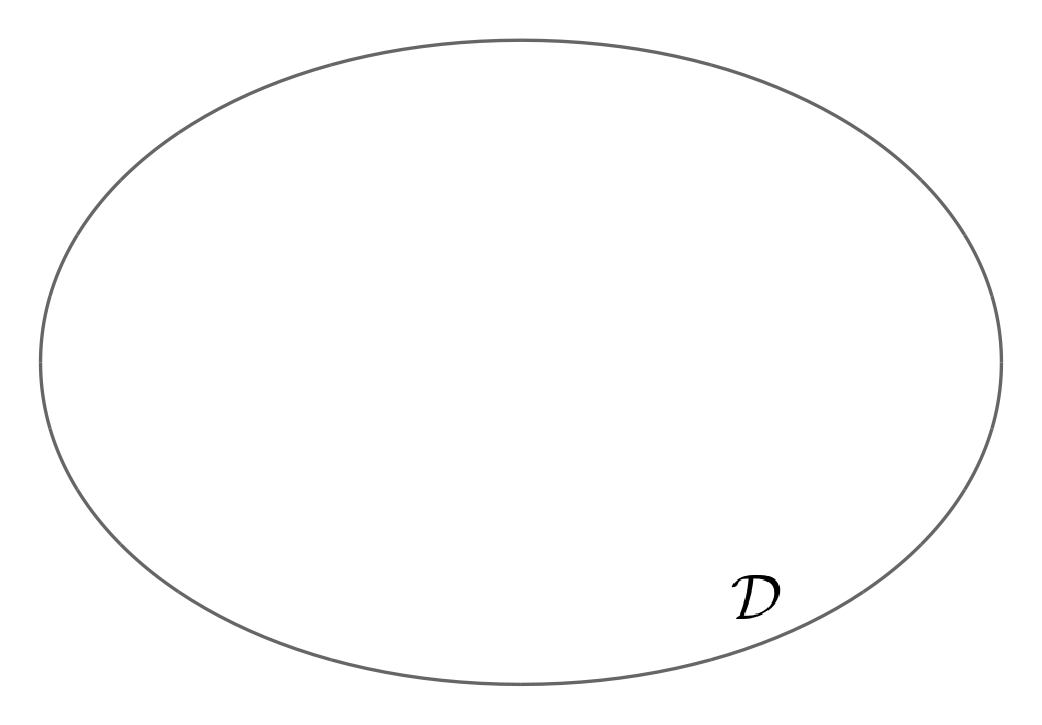
\includegraphics[scale=0.26]{pics/vi1.png}
\end{frame}

\begin{frame}
\thetitle{Variational Inference \citep{Jordan1999}}
$\mathcal{D}$: All distributions over $z$ \\
\color{white}{$\mathcal{Q}$: Variational family }
\center
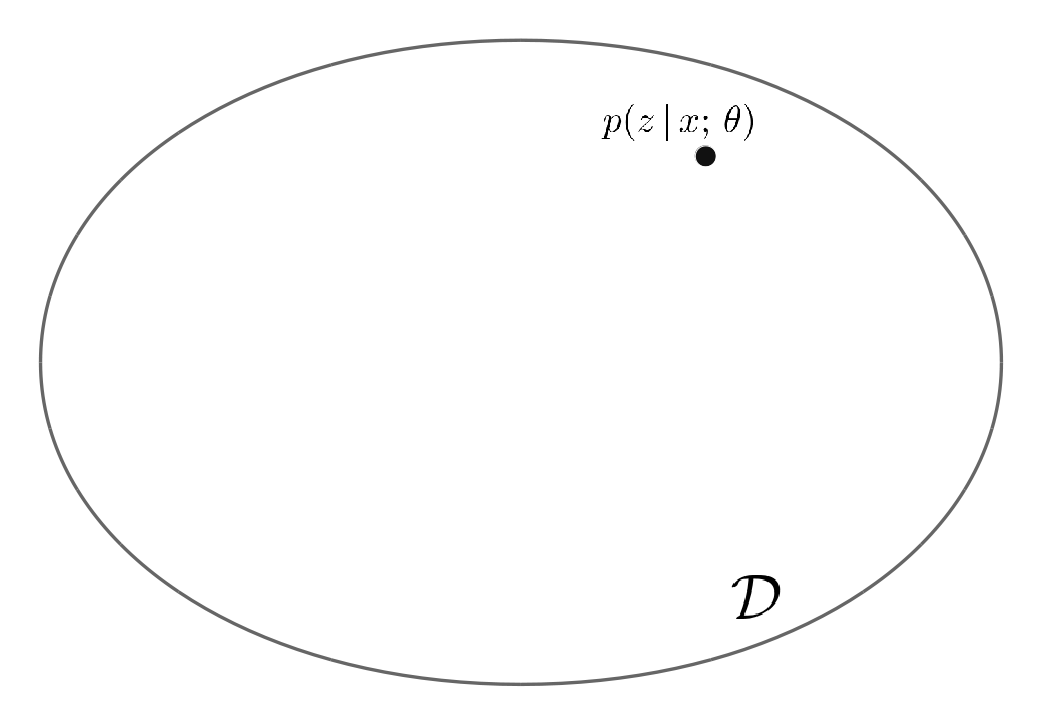
\includegraphics[scale=0.26]{pics/vi2.png}
\end{frame}

\begin{frame}
\thetitle{Variational Inference \citep{Jordan1999}}
$\mathcal{D}$: All distributions over $z$ \\
$\mathcal{Q}$: Variational family 
\center
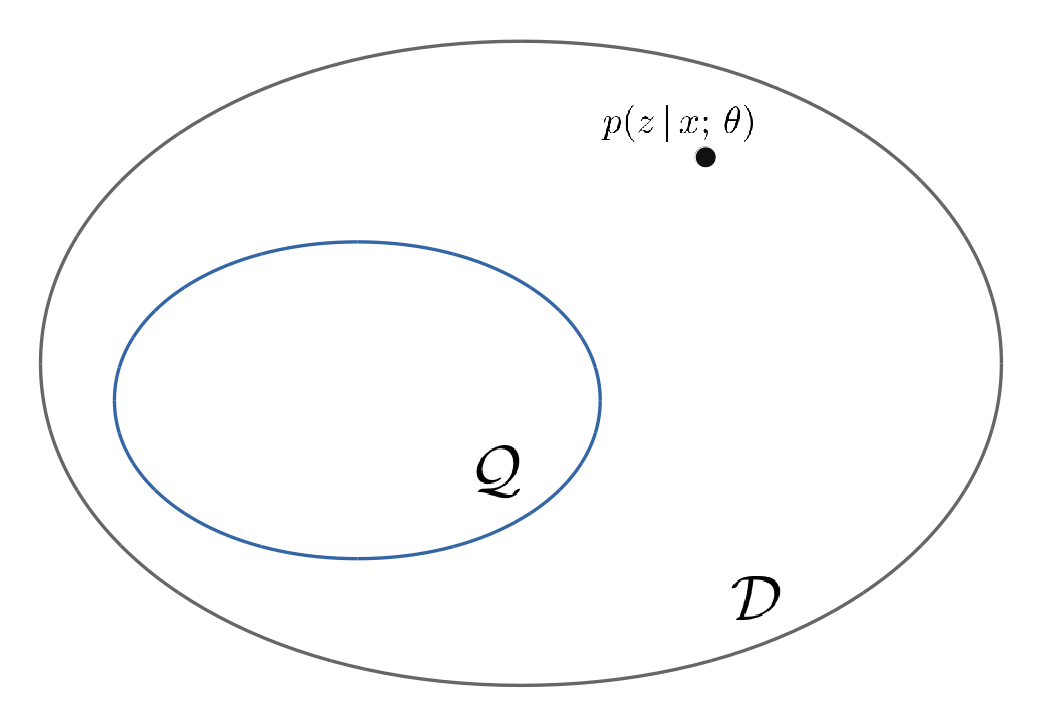
\includegraphics[scale=0.26]{pics/vi3.png}
\end{frame}

\begin{frame}
\thetitle{Variational Inference \citep{Jordan1999}}
$\mathcal{D}$: All distributions over $z$ \\
$\mathcal{Q}$: Variational family 
\center
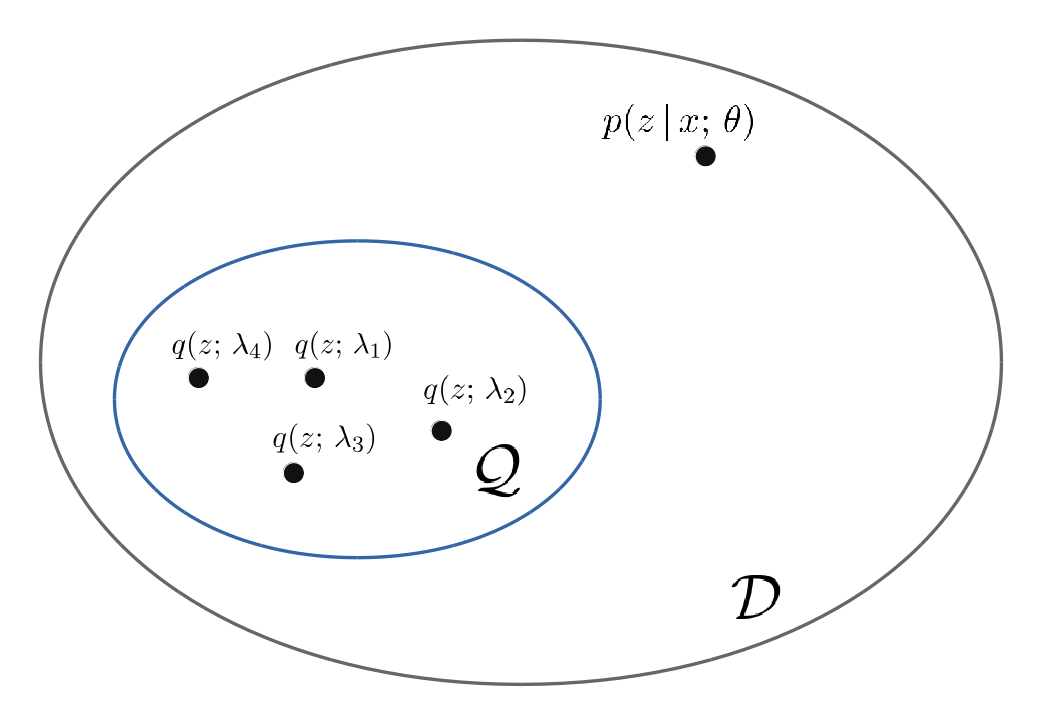
\includegraphics[scale=0.26]{pics/vi4.png}
\end{frame}

\begin{frame}
\thetitle{Variational Inference \citep{Jordan1999}}
$\mathcal{D}$: All distributions over $z$ \\
$\mathcal{Q}$: Variational family 
\center
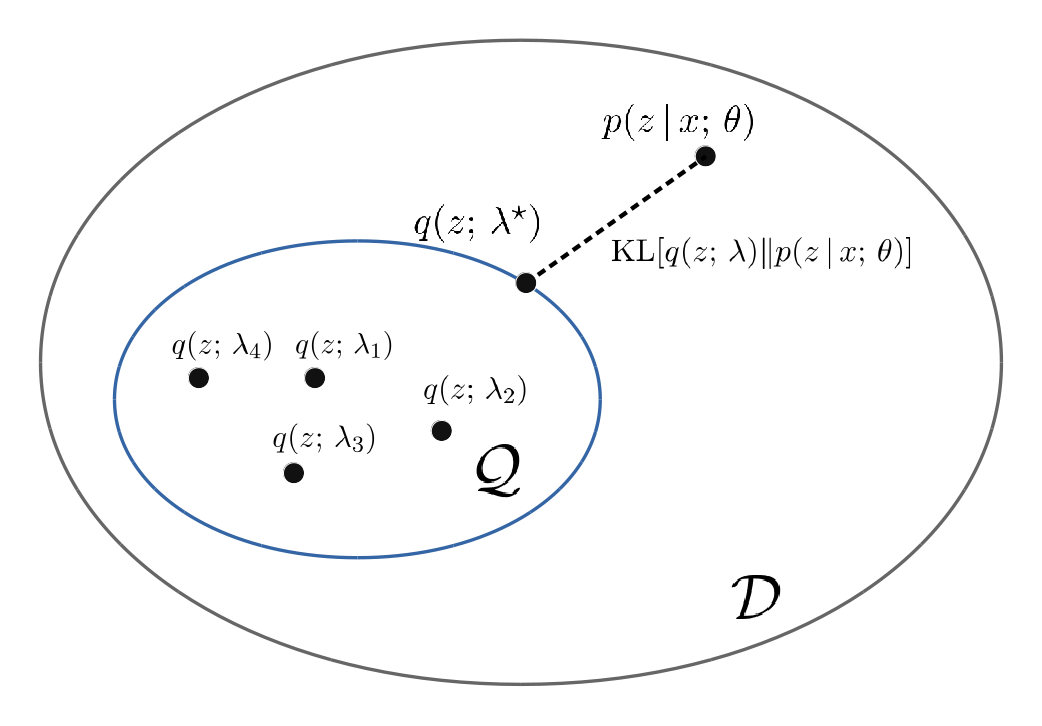
\includegraphics[scale=0.26]{pics/vi5.png}
\end{frame}


\begin{frame}
\thetitle{Variational EM \citep{neal1998}}
Assume for now we can efficiently minimize $\KL [q(z \param \lambda) \Vert p(z \given x^{(n)} \param \theta)]$ for each $x^{(n)}$

\begin{enumerate}
    \item Inference Step: For $n = 1, \dots, N$, calculate the approximate posterior $q(z  \param \lambda^{(n)})$ keeping $\theta^{(i)}$ fixed
    \[ \lambda^{(n)} = \argmin_{\lambda: q(z \param \lambda) \in \mathcal{Q}} \KL [q(z \param \lambda) \Vert p(z \given x^{(n)} \param \theta^{(i)})]\]
    \item Learning Step: Keeping $\lambda^{(n)}$'s fixed, maximize the expected complete data likelihood 
    \[ \theta^{(i+1)} = \argmax_{\theta} \sum_{n=1}^N \E_{q(z \param \lambda^{(n)})}[\log p(x, z \param \theta)] \]
    (can also approximately maximize)
\end{enumerate}
\end{frame}

\begin{frame}
\thetitle{Recap}
\vspace{-3mm}
\begin{table}[]
    \centering
    \begin{tabular}{l c c }
    \toprule
        Optimization Method  & Inference & Learning \\
    \midrule
         Expectation Maximization & Exact Post. & Exact \\
         Log Marginal Likelihood & Exact Post. & Gradient \\
         Variational EM & VI & Exact/Gradient \\
         {\color{white} Stochastic Variational EM} & {\color{white} SVI} & {\color{white} Gradient}\\
         {\color{white} Variational Autoencoder} & {\color{white} AVI} & {\color{white} Gradient} \\
         \bottomrule
    \end{tabular}
\end{table}
\end{frame}


\begin{frame}
\thetitle{Stochastic Variational Inference \citep{Hoffman2013}}
\begin{itemize}
    \item Exact variational inference 
\[ \lambda^{(n)} = \argmin_{\lambda : q(z \param \lambda) \in \mathcal{Q}} \KL[q(z \param \lambda)  \, \Vert \, p(z \given x^{(n)} \param \theta)]\]
could be expensive/slow.
\item Stochastic variational inference (SVI): approximately minimize KL with (for example) gradient descent.
\item Approximate approximate inference.
\end{itemize}
\end{frame}

\begin{frame}
\thetitle{Stochastic Variational Inference \citep{Hoffman2013}}

\textbf{Stochastic Variational EM}
\begin{enumerate}
    \item Randomly initialize $\lambda^{(n)}_0$ for all $n$ (usually over mini-batch)
    \item $K$-steps of gradient descent for each $x^{(n)}$
    \[ \lambda_{k}^{(n)} = \lambda_{k-1}^{(n)} + \eta \nabla_\lambda \ELBO(\theta^{(i)}, \lambda^{(n)}_{k-1} \param x^{(n)}) \]
    \item Update $\theta$
    \[ \theta^{(i+1)} = \theta^{(i)} + \eta \sum_{n=1}^N \nabla_\theta \ELBO(\theta^{(i)}, \lambda^{(n)}_K \param x^{(n)}) \]
\end{enumerate}
\end{frame}

\begin{frame}
\thetitle{Recap}
\vspace{-3mm}
\begin{table}[]
    \centering
    \begin{tabular}{l c c }
    \toprule
        Optimization Method  & Inference & Learning \\
    \midrule
         Expectation Maximization & Exact Post. & Exact \\
         Log Marginal Likelihood & Exact Post. & Gradient \\
         Variational EM & VI & Exact/Gradient \\
         Stochastic Variational EM & SVI &  Gradient\\
         {\color{white} Variational Autoencoder} & {\color{white} AVI} & {\color{white} Gradient} \\
         \bottomrule
    \end{tabular}
\end{table}
\end{frame}

\begin{frame}
\thetitle{Amortized Variational Inference \citep{Kingma2014}}
\begin{itemize}
    \item SVI allows for faster inference since we can approximately perform VI with 
    gradient ascent.
    \item But this could still be too slow, since each SVI step requires calculating the gradient $ \nabla_\lambda \ELBO(\theta^{(i)}, \lambda^{(n)}_{k-1} \param x^{(n)})$ for each data point.
    \item Amortized Variational Inference: \\
    \textbf{Predict} the variational parameters from a parametric function over $x$
\end{itemize}
\end{frame}

\begin{frame}
\thetitle{Amortized Variational Inference \citep{Kingma2014}}
Define an \textbf{inference network} parameterized by $\phi$. Variational parameters for each data point
are given by
\[ \lambda^{(n)} = \enc(x^{(n)} \param \phi)\]
\begin{itemize}
    \item $\phi$ trained via SGD to perform inference
    \[ \phi = \phi + \eta \nabla_\phi \sum_{n=1}^B \ELBO(\theta, \enc(x^{(n)} \param \phi) \param x^{(n)})\]
    \item Since a \textbf{global} inference network $\phi$ is used for all $x^{(n)}$, we say that the approximate posterior inference procedure is \textbf{amortized} across the dataset.
\end{itemize}
\end{frame}

\begin{frame}
\thetitle{Amortized Variational Inference \citep{Kingma2014}}
$\mathcal{D}$: All distributions over $z$ \\
$\mathcal{Q}$: Variational family \\
{\color{white} $\mathcal{Q}_\phi$: Amortized Variational family }
\center
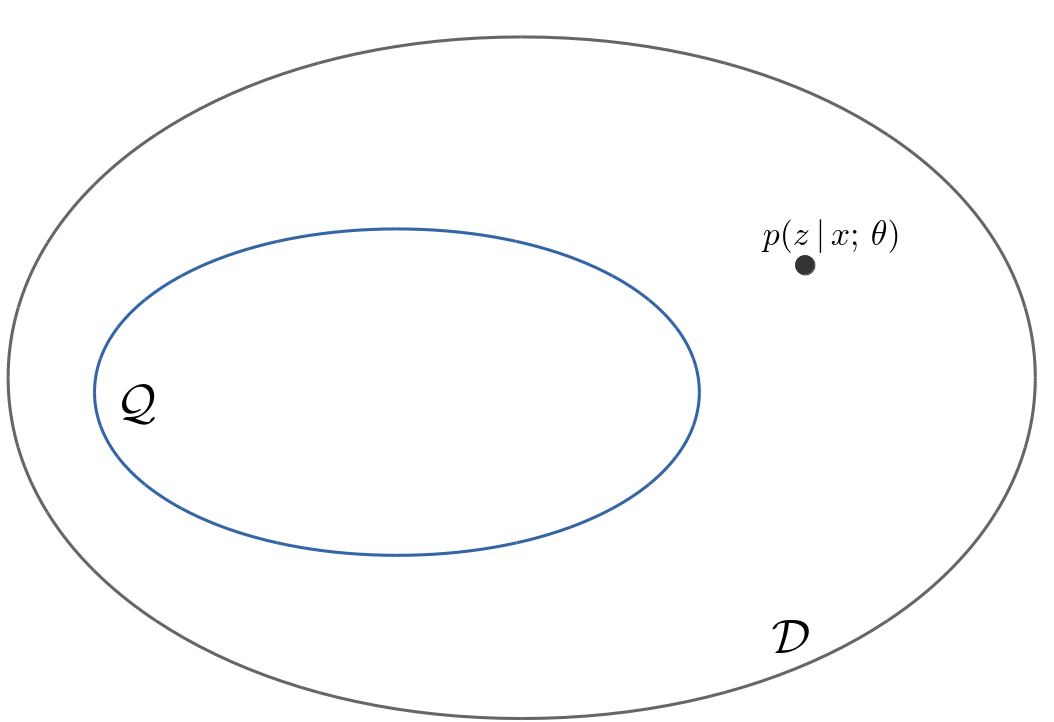
\includegraphics[scale=0.24]{pics/avi1.png}
\end{frame}
 
 
\begin{frame}
\thetitle{Amortized Variational Inference \citep{Kingma2014}}
$\mathcal{D}$: All distributions over $z$ \\
$\mathcal{Q}$: Variational family \\
{\color{white} $\mathcal{Q}_\phi$: Amortized Variational family }
\center
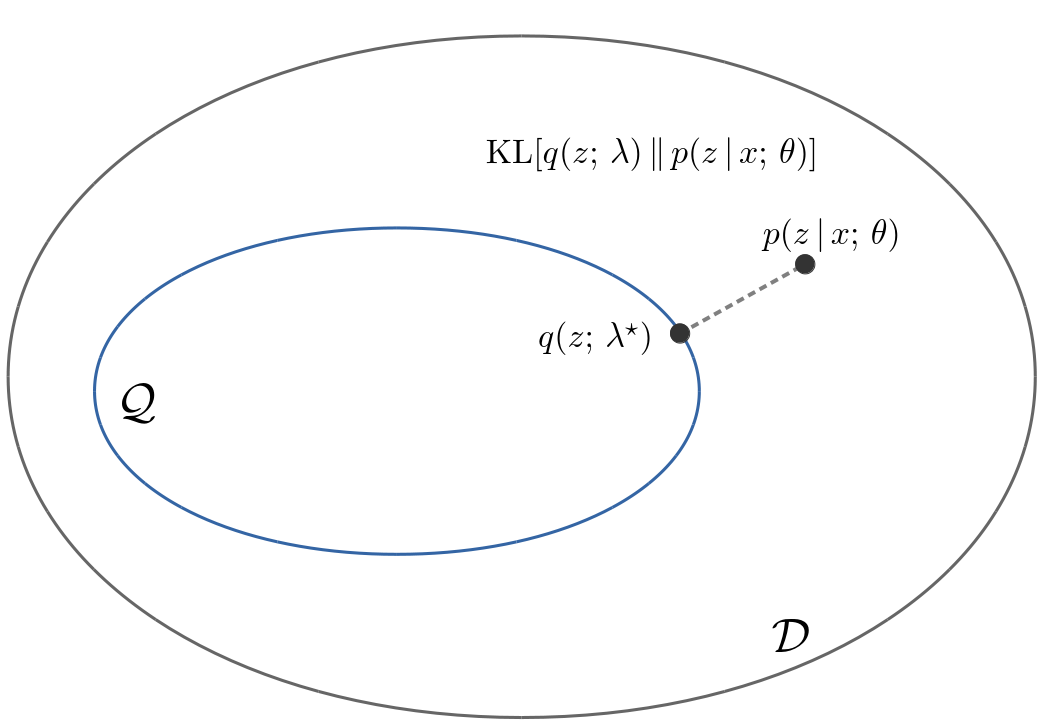
\includegraphics[scale=0.24]{pics/avi2.png}
\end{frame}
 
\begin{frame}
\thetitle{Amortized Variational Inference \citep{Kingma2014}}
$\mathcal{D}$: All distributions over $z$ \\
$\mathcal{Q}$: Variational family \\
$\mathcal{Q}_\phi$: Amortized Variational family 
\center
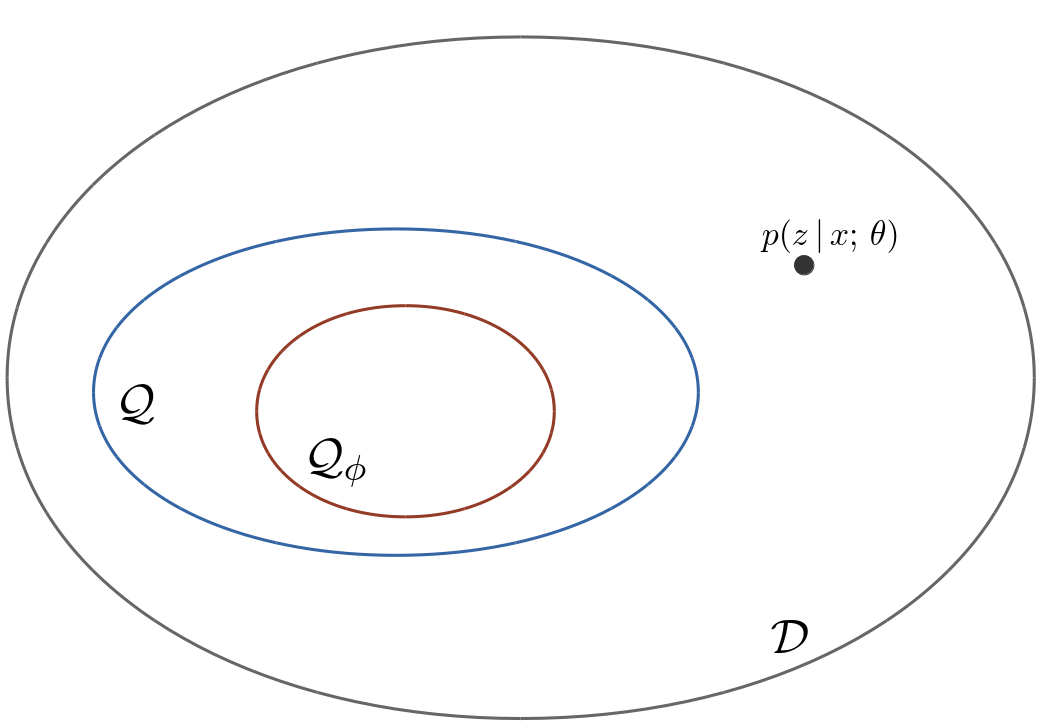
\includegraphics[scale=0.24]{pics/avi3.png}
\end{frame}
  
\begin{frame}
\thetitle{Amortized Variational Inference \citep{Kingma2014}}
$\mathcal{D}$: All distributions over $z$ \\
$\mathcal{Q}$: Variational family \\
$\mathcal{Q}_\phi$: Amortized Variational family 
\center
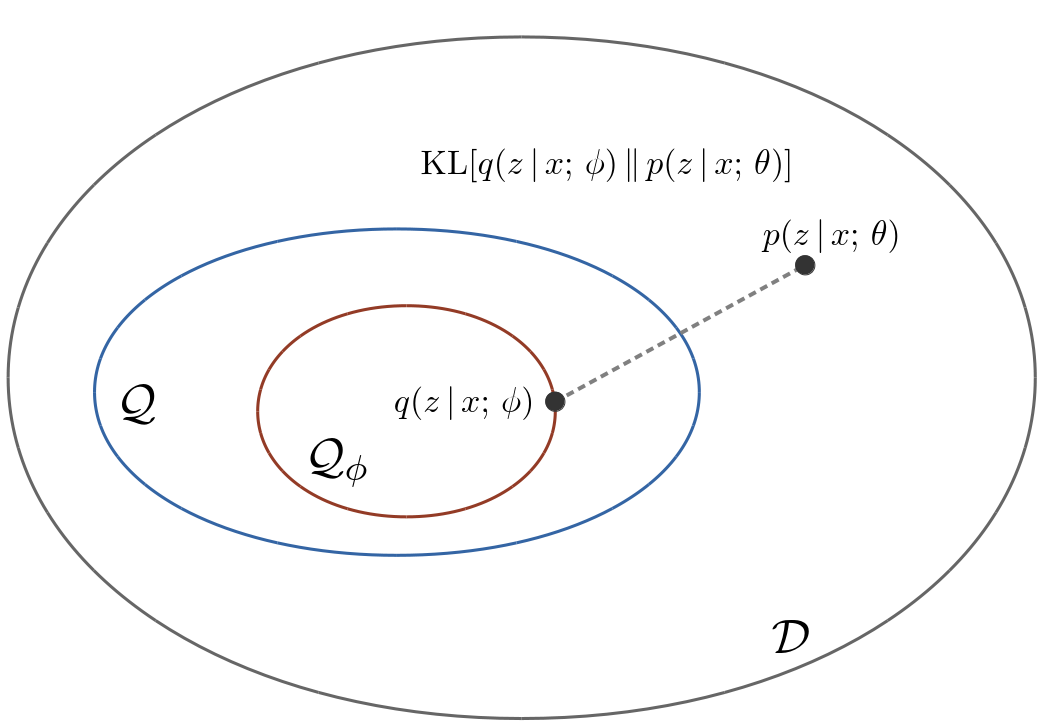
\includegraphics[scale=0.24]{pics/avi4.png}
\end{frame}

 
\begin{frame}
\thetitle{Variational Autoencoders \citep{Kingma2014}}
\begin{itemize}
    \item Deep generative models trained with amortized inference
    \item Generative model $\theta$ and inference network $\phi$ trained \textbf{jointly} to maximize the aggregate ELBO
    \[L(\theta, \phi) =  \sum_{n=1}^N \ELBO(\theta, \phi \param x^{(n)})\]
    \item Typically trained with gradient-based optimization over mini-batches
    \begin{align*}
        \theta &= \theta + \eta \nabla_\theta L(\theta, \phi) \\
        \phi &= \phi + \eta \nabla_\phi L(\theta, \phi)
    \end{align*}
\end{itemize}
\end{frame}

\begin{frame}
\thetitle{Why ``autoencoder"?}
\begin{align*}
    &\ELBO(\theta, \phi \param x ) = \E_{q(z \given x \param \phi)}\Big[\log \frac{p(x, z \param \theta)}{q(z \given x \param \phi)}\Big] \\
    &= \E_{q(z \given x \param \phi)}[\log p( x \given z \param \theta) + \log p(z) - \log q(z \given x \param \phi)] \\
        &= \E_{q(z \given x \param \phi)}[\log p( x \given z \param \theta)] - \E_{q(z \given x \param \phi)}\Big[\log \frac{q(z \given x \param \phi)}{p(z)} \Big] \\
        &= \E_{q(z \given x \param \phi)}[\log p( x \given z \param \theta)] - \KL[q(z \given x \param \phi) \Vert p(z)]
\end{align*}
\end{frame}


\begin{frame}
\thetitle{Why ``autoencoder"?}
\begin{align*}
    &\ELBO(\theta, \phi \param x )  = \E_{q(z \given x \param \phi)}\Big[\log \frac{p(x, z \param \theta)}{q(z \given x \param \phi)}\Big] \\
    &= \E_{q(z \given x \param \phi)}[\log p( x \given z \param \theta) + \log p(z) - \log q(z \given x \param \phi)] \\
        &= \E_{q(z \given x \param \phi)}[\log p( x \given z \param \theta)] - \E_{q(z \given x \param \phi)}\Big[\log \frac{q(z \given x \param \phi)}{p(z)} \Big] \\
        &= \underbrace{\E_{q(z \given x \param \phi)}[\log p( x \given z \param \theta)]}_{\text{AE reconstruction likelihood}} - \underbrace{\KL[q(z \given x \param \phi) \Vert p(z)]}_{\text{Regularize posterior to prior}}
\end{align*}
\end{frame}


\begin{frame}
\thetitle{Recap}

\begin{table}[]
    \centering
    \begin{tabular}{l c c }
    \toprule
        Optimization Method  & Inference & Learning \\
    \midrule
         Expectation Maximization & Exact Post. & Exact \\
         Log Marginal Likelihood & Exact Post. & Gradient \\
         Variational EM & VI & Exact/Gradient \\
         Stochastic Variational EM & SVI & Gradient\\
         Variational Autoencoder & AVI & Gradient \\
         \bottomrule
    \end{tabular}
\end{table}
\vspace{-3mm}
\textbf{Inference Methods} \\
Exact Posterior: $q(z \param \lambda ) = p(z \given x \param \theta)$ \\
Variational Inference (VI): $\lambda = \argmax_\lambda \ELBO(\theta, \lambda \param x) $ \\
%=\min_\lambda \KL[q(z \param \lambda) \Vert p(z \given x \param \theta)]$ \\
Stochastic VI: $\lambda = \lambda + \eta \nabla_\lambda \ELBO(\theta, \lambda \param x)$ \\
Amortized VI: $\lambda = \enc(x \param \phi) $
\end{frame}
